\documentclass[ngerman]{scrartcl}

\KOMAoptions{fontsize=11pt,paper=a4}
\KOMAoptions{DIV=14}

\usepackage{babel}
\usepackage[utf8]{inputenc}
\usepackage[T1]{fontenc}
\usepackage[autostyle=true]{csquotes}
\usepackage{amsmath}
\usepackage[varg]{txfonts}
\usepackage{graphicx}
\usepackage{hyperref}

\graphicspath{{figs/}}

\begin{document}

\title{Übungsblatt 1 zur Vorlesung 'Numerische Methoden der Physik' SS 2015}
\subtitle{Madelung-Energie des NaCl-Kristalls}
\author{Fabian Schmidt und Marvin Schmitz}
\maketitle

\newpage

\section*{Physikalische Beschreibung des Problems}

Wir betrachten ein NaCl-Kristallgitter. Wir wollen die Energie eines Ions im Kristallgitter numerisch bestimmen.
Dies wollen wir durch Summation der Einzelbeiträge erreichen: \\ \\
$ V_{i,j} = \frac{1}{4\pi \epsilon_0} \cdot \frac{e_ie_j}{r_i,j}\ \ mit\ \ r_{i,j} = a\cdot \sqrt{(i_1-j_1)^2+(i_2-j_2)^2+(i_3-j_3)^2} $\\ \\
Dabei ist a der Gitterabstand und $e_{i,j}$ jeweils positiv für ein Kation und negativ für ein Anion. Die gewünschte Genauigkeit der Approximation soll $10^{-5}$ sein. Desweiteren betrachten wir zusätzlich nochmal den Fall eines flachen Kristallgitters also $i_3=j_3$.

\section*{Modellierung des Problems}

Berechnet werden soll die Madelung-Energie. Dazu führen wir die Madelung-Konstante ein. Sei $E_{IP}$ die Energie eines Ions im Ionenpaar und $E_{IG}$ die Energie eines Ions im Gitter, dann ergibt sich:\\ \\
$ E_{IG} = n_1 \cdot \frac{E_{IP}}{c_1} + n_2\cdot \frac{E_{IP}}{c_2} + n_3\cdot \frac{E_{IP}}{c_3} + ... $ \\ \\
Wobei $c_1$ ein für den Abstand des Ions spezifische Konstante ist und $n_1$ die Häufigkeit des Ions (Quelle: Wikipedia Madelung-Konstante). Diese Konstanten kann man zusammenfassen zu der Madelung-Konstante:\\ \\
$ E_{IG} = \alpha \cdot E_{IP} $\\ \\
Damit ergibt sich dann die Madelung-Konstante als Summe. Um die Kristallstruktur des NaCl besser zu berücksichtigen stellen wir uns die Ionen kubisch angeordnet vor. Wir betrachten also ein Ion, welches wir mit 0 kennzeichnen und bilden n-Würfel um das 0-te Ion herum. Auf diesen Würfeln befinden sich dann die Ionen, die wir bezüglich ihres Abstandes und ihrer Ladung mit 1, 2, 3, ... klassifizieren. (siehe Abb) Weiterhin berücksichtigen wir, das die Ionen auf dem aüßersten Rand eines Würfels nur zu $ 1/8 $ an den Ecken zu einem $ 1/4 $ an den Kanten und zu $ 1/2 $ auf der Fläche beitragen.

\begin{figure}[H]
\centering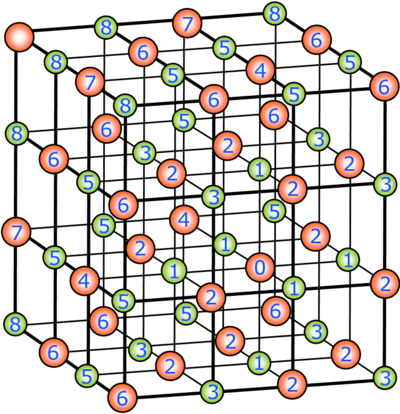
\includegraphics[width=9cm]{madelung}
\end{figure}


\section*{Implementierung der Lösung}

% an Fabian: ich weiß ja nicht was du noch änderst ... 
Unser Programm ist folgendermassen aufgebaut. Wir berechnen mit einer Funktion madelung2dim(int n)  bzw. madelung3dim(int n) die Madelung Konstante über Summations der Einzelbeträge. Dabei ist int n die Größe des würfels. Wir unterscheiden zusätzlich ob sich das jeweilige Ion auf dem Rand befindet und wenn ja wo. Die Beiträge dieser Ionen werden dann mit dem oben diskutierten Faktoren gewichtet.
\\
Die zweite Funktion bindungsenergieint(int dim, double d, double var) ist dafür da die Energie letzendlich zu berechen. Ihr übergeben wir die Dimension (flach, 3dim), welche letzlich entscheidet, ob die Madelung-Konstante mit madelung2dim oder madelung3dim berechnet wird. Weitere Parameter sin die Gitterkonstante (double d) und die Genauigkeit (double var). Die Genauigkeit der berechneten Energie wird mittels einer while-Schleife und dem Parameter double var bestimmt. Wir berechen die Energie für einen Würfel mit n und mit n+1 und prüfen, ob der Wert $ \frac{E_{n+1}}{E_n} > var $ ist. Wenn die Bedingung erfüllt ist wird n um eins erhöht. Die Energie berechnet sich zu
$ E = \alpha \cdot 1/{4\pi\epsilon_0} $. Der dadurch erhaltene Wert für die Madelungsenergie wird in der Funktion int main() in die Variable double Energie gespeichert und ausgegeben.


\end{document}